\documentclass[12pt, specialist, subf, substylefile = spbu.rtx]{disser}
\usepackage[a4paper, includefoot,
            left=3cm, right=1.5cm,
            top=2cm, bottom=2cm,
            headsep=1cm, footskip=1cm]{geometry}
\usepackage[utf8]{inputenc}
\usepackage[T1, T2A]{fontenc}
\usepackage[english, russian]{babel}
\usepackage{moreverb}
\usepackage{array}
\usepackage{hyperref}
\usepackage{amsthm}

\makeatletter
\newcommand{\@chapapp}{\relax}
\makeatother

\usepackage[title,toc,titletoc,header]{appendix}
\setcounter{tocdepth}{2}
\graphicspath{{diploma3_fig/}}
\newtheorem{theorem}{Теорема}
\newtheorem{definition}{Определение}
\newtheorem{algo}{Алгоритм}
\newcommand{\Expect}{\mathsf{E}}
\newcommand{\CVaR}{\mathsf{CVaR}}
\newcommand{\Var}{\mathsf{Var}}
\DeclareGraphicsExtensions{.pdf,.png}
\DeclareMathOperator*{\toplim}{\overline\lim}
\DeclareMathOperator*{\botlim}{\underline\lim}
\DeclareMathOperator*{\tou}{\longrightarrow}
\newcommand{\MDA}{\mathsf{MDA}}
\begin{document}

Прямая оценка. Имеем:

$$
b_n=b_n(\gamma)=\frac{N^{-1}(\gamma)}{\sqrt{z}\sigma_T},
$$
где $N^{-1}$ -- обратная функция стд. нормального распределения;
$z$ -- количество выборок, по которым будет строиться оценка вероятности, $\sigma_T$ -- ср.кв. отклонение для функционала. Вид функционала:

$$
T=\hat{\alpha}_H^{-1}=\frac{1}{n-m+1}\sum_{i=m}^n Y_{i:n}-Y_{m:n},
$$
$Y_i \sim exp(\alpha)$, $n$ -- количество измерений, для которых строится одна оценка $\hat{\alpha}_H^{-1}$.

Далее, берется диапазон $\gamma_k \in [0.9, 1]$ с некоторым шагом, для каждого $\gamma_k$ считается оценка вероятности:
$$
\hat{\omega}_k = \frac{\#\left(\hat{\alpha}_H(Y)^{-1}-\alpha^{-1} > b_n(\gamma_k)  \right)}{z}
$$
На каждом шаге генерируется новая выборка $Y$.

График строится в осях $\hat{\omega}_k$ и $\gamma$. Пример графика для $\alpha=1, \frac{m}{n}=0.75, z=1000, n=1000$


\begin{figure}[!h]
\center{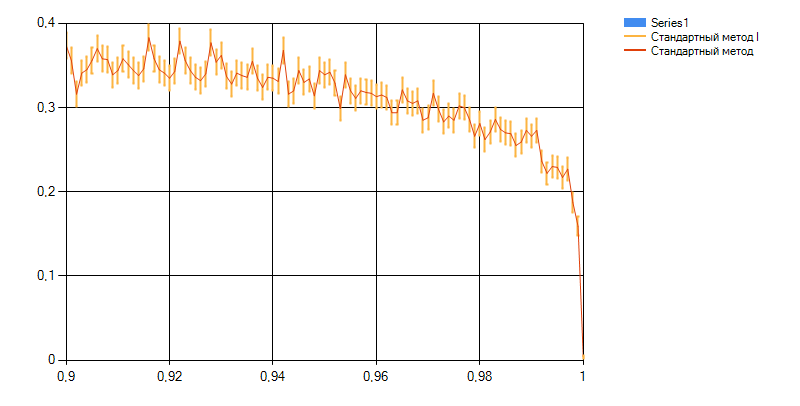
\includegraphics[width=1\linewidth]{hhnz}}
\label{ris:hhnz}
\end{figure}



  











\end{document}